% Demonstration homework, built from real EECS 16A material.
%
% Build both variants from this ONE source. The class option is NOT written
% here, so build.sh can supply it:
%   pdflatex "\PassOptionsToClass{sol}{latexa11y-assignment}% Demonstration homework, built from real EECS 16A material.
%
% Build both variants from this ONE source. The class option is NOT written
% here, so build.sh can supply it:
%   pdflatex "\PassOptionsToClass{sol}{latexa11y-assignment}% Demonstration homework, built from real EECS 16A material.
%
% Build both variants from this ONE source. The class option is NOT written
% here, so build.sh can supply it:
%   pdflatex "\PassOptionsToClass{sol}{latexa11y-assignment}% Demonstration homework, built from real EECS 16A material.
%
% Build both variants from this ONE source. The class option is NOT written
% here, so build.sh can supply it:
%   pdflatex "\PassOptionsToClass{sol}{latexa11y-assignment}\input{demo-homework}"
%   pdflatex "\PassOptionsToClass{prob}{latexa11y-assignment}\input{demo-homework}"
% Hard-coding [sol] below would make `prob` a no-op, because both options would
% be processed and whichever \DeclareOption runs last wins.
%
% Open the result in a PDF reader and look at the bookmark/navigation pane:
% Homework 9 > Question 1 > Part (a) > Solution. Then run a screen reader over
% the figures: each is announced by its description, never by its contents.

\DocumentMetadata{
  lang       = en-US,
  pdfversion = 2.0,
  testphase  = {phase-III,math,table,graphic,firstaid},
}
\documentclass{latexa11y-assignment}

\usepackage{tikz}
\usepackage{pgfplots}
\pgfplotsset{compat=1.16}
\usepackage[american]{circuitikz}

\coursenumber{EECS 16A}
\coursename{Designing Information Devices and Systems I}
\semester{Spring 2026}
\university{UC Berkeley}

\begin{document}

\title{Homework 9}
\maketitle

\noindent
This homework is due Friday, April 3, 2026, at 23:59. Self-grades are due
Monday, April 6, 2026, at 23:59.

% ----------------------------------------------------------------------------
\question{Capacitor Charge Sharing}

Two capacitors are connected through a switch. Before $t=0$ the switch $S_1$ is
open, capacitor $C_1$ is charged to $V_1(0) = 5$\,V, and $C_2$ is uncharged.

% The figure speaks ONLY the description below. The labels drawn inside the
% schematic are never announced.
\begin{AltOnly}{Two capacitors, C1 and C2, each connected from its own top node
to ground, with switch S1 joining the two top nodes. C1 carries voltage V1 and
C2 carries voltage V2, both positive at the top.}
\begin{center}
\begin{circuitikz}[scale=0.9]
  \draw (0, 0) node[ground]{}
    (0, 3) to [C=$C_1$, v=$V_1$] ++ (0, -3)
    (0, 3) to [switch, l=$S_1$] ++ (6, 0)
          to [C=$C_2$, v=$V_2$] ++ (0, -3)
    node[ground]{};
\end{circuitikz}
\end{center}
\end{AltOnly}

\questionpart[5]
Express the total charge stored on both capacitors immediately before the
switch closes.

\begin{solution}
Only $C_1$ is charged, so $Q_{\text{total}} = C_1 V_1(0)$.
\end{solution}

\questionpart[5]
Find the steady-state voltage across both capacitors after the switch closes.

\begin{solution}
Charge is conserved and the two capacitors share a node, so they settle to a
common voltage
\[
  V_\infty = \frac{C_1 V_1(0)}{C_1 + C_2}.
\]
\end{solution}

% ----------------------------------------------------------------------------
\question{Least Squares Fit}

The table below records four measurements. A best-fit line has already been
drawn through them.

% Short /Alt plus a visible long description and a real data table: the tier
% for a figure whose data cannot fit in one spoken sentence.
\begin{FigureBlock}[alt={Scatter plot of b against a on axes running 0 to 9,
with four measured points and a straight best-fit line.}]
\begin{center}
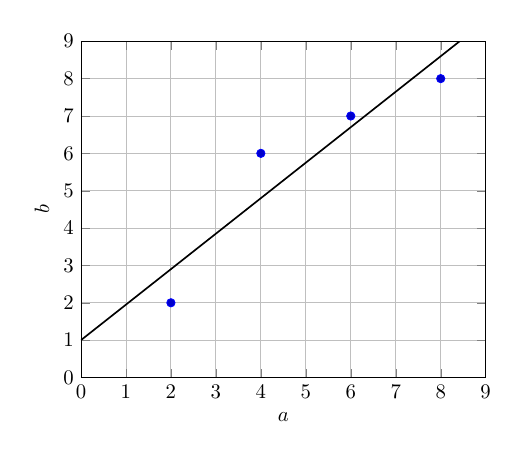
\begin{tikzpicture}[scale=0.75]
\begin{axis}[xlabel=$a$, ylabel=$b$, xmin=0, xmax=9, ymin=0, ymax=9,
             xtick={0,1,...,9}, ytick={0,1,...,9}, grid=major]
  \addplot+[only marks, mark=*] coordinates {(2,2) (4,6) (6,7) (8,8)};
  \addplot[thick, domain=0:9]{0.95 * x + 1};
\end{axis}
\end{tikzpicture}
\end{center}
\end{FigureBlock}
\FigureDescription{Horizontal axis $a$ runs from 0 to 9 with integer ticks;
vertical axis $b$ runs from 0 to 9 with integer ticks. The fitted line is
$b = 0.95a + 1$, passing through 1 at $a=0$ and 9.55 at $a=9$. It lies above
the first measured point and below the third.}

\begin{DataTable}[table/header-rows={1}]
\begin{center}
\begin{tabular}{|c|c|}
\hline
$a$ & $b$ \\
\hline
2 & 2 \\
4 & 6 \\
6 & 7 \\
8 & 8 \\
\hline
\end{tabular}
\end{center}
\end{DataTable}

\questionpart[10]
Set up the normal equations for the least-squares fit and solve for the slope
and intercept.

\begin{solution}
With $\mathbf{A}$ the matrix whose rows are $[a_i \;\; 1]$ and $\vec{b}$ the
vector of measurements, the normal equations are
$\mathbf{A}^{\!\top}\mathbf{A}\,\vec{x} = \mathbf{A}^{\!\top}\vec{b}$, giving a
slope of $0.95$ and an intercept of $1$.
\end{solution}

% ----------------------------------------------------------------------------
\question{Written Response}

\questionpart
State, in one sentence, why the residuals of a least-squares fit must be
orthogonal to the column space of $\mathbf{A}$.

% A tagged answer region, announced as such. The corpus used
% \framebox(470,42){} here, which is picture-mode and carries no semantics.
\answerbox[4\baselineskip]

\end{document}
"
%   pdflatex "\PassOptionsToClass{prob}{latexa11y-assignment}% Demonstration homework, built from real EECS 16A material.
%
% Build both variants from this ONE source. The class option is NOT written
% here, so build.sh can supply it:
%   pdflatex "\PassOptionsToClass{sol}{latexa11y-assignment}\input{demo-homework}"
%   pdflatex "\PassOptionsToClass{prob}{latexa11y-assignment}\input{demo-homework}"
% Hard-coding [sol] below would make `prob` a no-op, because both options would
% be processed and whichever \DeclareOption runs last wins.
%
% Open the result in a PDF reader and look at the bookmark/navigation pane:
% Homework 9 > Question 1 > Part (a) > Solution. Then run a screen reader over
% the figures: each is announced by its description, never by its contents.

\DocumentMetadata{
  lang       = en-US,
  pdfversion = 2.0,
  testphase  = {phase-III,math,table,graphic,firstaid},
}
\documentclass{latexa11y-assignment}

\usepackage{tikz}
\usepackage{pgfplots}
\pgfplotsset{compat=1.16}
\usepackage[american]{circuitikz}

\coursenumber{EECS 16A}
\coursename{Designing Information Devices and Systems I}
\semester{Spring 2026}
\university{UC Berkeley}

\begin{document}

\title{Homework 9}
\maketitle

\noindent
This homework is due Friday, April 3, 2026, at 23:59. Self-grades are due
Monday, April 6, 2026, at 23:59.

% ----------------------------------------------------------------------------
\question{Capacitor Charge Sharing}

Two capacitors are connected through a switch. Before $t=0$ the switch $S_1$ is
open, capacitor $C_1$ is charged to $V_1(0) = 5$\,V, and $C_2$ is uncharged.

% The figure speaks ONLY the description below. The labels drawn inside the
% schematic are never announced.
\begin{AltOnly}{Two capacitors, C1 and C2, each connected from its own top node
to ground, with switch S1 joining the two top nodes. C1 carries voltage V1 and
C2 carries voltage V2, both positive at the top.}
\begin{center}
\begin{circuitikz}[scale=0.9]
  \draw (0, 0) node[ground]{}
    (0, 3) to [C=$C_1$, v=$V_1$] ++ (0, -3)
    (0, 3) to [switch, l=$S_1$] ++ (6, 0)
          to [C=$C_2$, v=$V_2$] ++ (0, -3)
    node[ground]{};
\end{circuitikz}
\end{center}
\end{AltOnly}

\questionpart[5]
Express the total charge stored on both capacitors immediately before the
switch closes.

\begin{solution}
Only $C_1$ is charged, so $Q_{\text{total}} = C_1 V_1(0)$.
\end{solution}

\questionpart[5]
Find the steady-state voltage across both capacitors after the switch closes.

\begin{solution}
Charge is conserved and the two capacitors share a node, so they settle to a
common voltage
\[
  V_\infty = \frac{C_1 V_1(0)}{C_1 + C_2}.
\]
\end{solution}

% ----------------------------------------------------------------------------
\question{Least Squares Fit}

The table below records four measurements. A best-fit line has already been
drawn through them.

% Short /Alt plus a visible long description and a real data table: the tier
% for a figure whose data cannot fit in one spoken sentence.
\begin{FigureBlock}[alt={Scatter plot of b against a on axes running 0 to 9,
with four measured points and a straight best-fit line.}]
\begin{center}
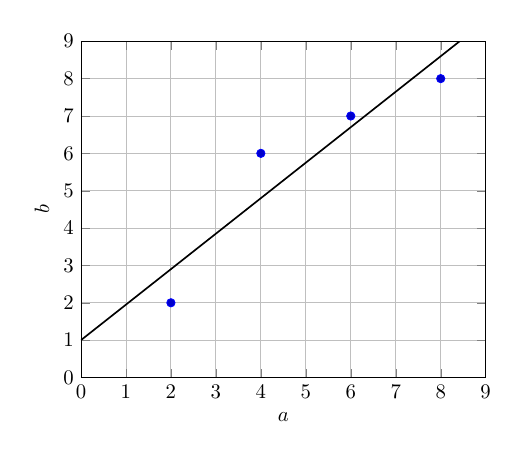
\begin{tikzpicture}[scale=0.75]
\begin{axis}[xlabel=$a$, ylabel=$b$, xmin=0, xmax=9, ymin=0, ymax=9,
             xtick={0,1,...,9}, ytick={0,1,...,9}, grid=major]
  \addplot+[only marks, mark=*] coordinates {(2,2) (4,6) (6,7) (8,8)};
  \addplot[thick, domain=0:9]{0.95 * x + 1};
\end{axis}
\end{tikzpicture}
\end{center}
\end{FigureBlock}
\FigureDescription{Horizontal axis $a$ runs from 0 to 9 with integer ticks;
vertical axis $b$ runs from 0 to 9 with integer ticks. The fitted line is
$b = 0.95a + 1$, passing through 1 at $a=0$ and 9.55 at $a=9$. It lies above
the first measured point and below the third.}

\begin{DataTable}[table/header-rows={1}]
\begin{center}
\begin{tabular}{|c|c|}
\hline
$a$ & $b$ \\
\hline
2 & 2 \\
4 & 6 \\
6 & 7 \\
8 & 8 \\
\hline
\end{tabular}
\end{center}
\end{DataTable}

\questionpart[10]
Set up the normal equations for the least-squares fit and solve for the slope
and intercept.

\begin{solution}
With $\mathbf{A}$ the matrix whose rows are $[a_i \;\; 1]$ and $\vec{b}$ the
vector of measurements, the normal equations are
$\mathbf{A}^{\!\top}\mathbf{A}\,\vec{x} = \mathbf{A}^{\!\top}\vec{b}$, giving a
slope of $0.95$ and an intercept of $1$.
\end{solution}

% ----------------------------------------------------------------------------
\question{Written Response}

\questionpart
State, in one sentence, why the residuals of a least-squares fit must be
orthogonal to the column space of $\mathbf{A}$.

% A tagged answer region, announced as such. The corpus used
% \framebox(470,42){} here, which is picture-mode and carries no semantics.
\answerbox[4\baselineskip]

\end{document}
"
% Hard-coding [sol] below would make `prob` a no-op, because both options would
% be processed and whichever \DeclareOption runs last wins.
%
% Open the result in a PDF reader and look at the bookmark/navigation pane:
% Homework 9 > Question 1 > Part (a) > Solution. Then run a screen reader over
% the figures: each is announced by its description, never by its contents.

\DocumentMetadata{
  lang       = en-US,
  pdfversion = 2.0,
  testphase  = {phase-III,math,table,graphic,firstaid},
}
\documentclass{latexa11y-assignment}

\usepackage{tikz}
\usepackage{pgfplots}
\pgfplotsset{compat=1.16}
\usepackage[american]{circuitikz}

\coursenumber{EECS 16A}
\coursename{Designing Information Devices and Systems I}
\semester{Spring 2026}
\university{UC Berkeley}

\begin{document}

\title{Homework 9}
\maketitle

\noindent
This homework is due Friday, April 3, 2026, at 23:59. Self-grades are due
Monday, April 6, 2026, at 23:59.

% ----------------------------------------------------------------------------
\question{Capacitor Charge Sharing}

Two capacitors are connected through a switch. Before $t=0$ the switch $S_1$ is
open, capacitor $C_1$ is charged to $V_1(0) = 5$\,V, and $C_2$ is uncharged.

% The figure speaks ONLY the description below. The labels drawn inside the
% schematic are never announced.
\begin{AltOnly}{Two capacitors, C1 and C2, each connected from its own top node
to ground, with switch S1 joining the two top nodes. C1 carries voltage V1 and
C2 carries voltage V2, both positive at the top.}
\begin{center}
\begin{circuitikz}[scale=0.9]
  \draw (0, 0) node[ground]{}
    (0, 3) to [C=$C_1$, v=$V_1$] ++ (0, -3)
    (0, 3) to [switch, l=$S_1$] ++ (6, 0)
          to [C=$C_2$, v=$V_2$] ++ (0, -3)
    node[ground]{};
\end{circuitikz}
\end{center}
\end{AltOnly}

\questionpart[5]
Express the total charge stored on both capacitors immediately before the
switch closes.

\begin{solution}
Only $C_1$ is charged, so $Q_{\text{total}} = C_1 V_1(0)$.
\end{solution}

\questionpart[5]
Find the steady-state voltage across both capacitors after the switch closes.

\begin{solution}
Charge is conserved and the two capacitors share a node, so they settle to a
common voltage
\[
  V_\infty = \frac{C_1 V_1(0)}{C_1 + C_2}.
\]
\end{solution}

% ----------------------------------------------------------------------------
\question{Least Squares Fit}

The table below records four measurements. A best-fit line has already been
drawn through them.

% Short /Alt plus a visible long description and a real data table: the tier
% for a figure whose data cannot fit in one spoken sentence.
\begin{FigureBlock}[alt={Scatter plot of b against a on axes running 0 to 9,
with four measured points and a straight best-fit line.}]
\begin{center}
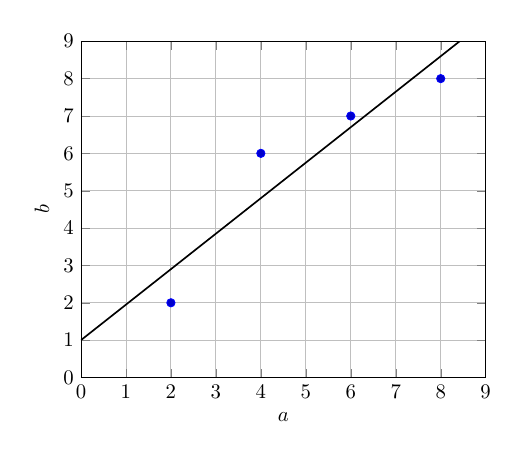
\begin{tikzpicture}[scale=0.75]
\begin{axis}[xlabel=$a$, ylabel=$b$, xmin=0, xmax=9, ymin=0, ymax=9,
             xtick={0,1,...,9}, ytick={0,1,...,9}, grid=major]
  \addplot+[only marks, mark=*] coordinates {(2,2) (4,6) (6,7) (8,8)};
  \addplot[thick, domain=0:9]{0.95 * x + 1};
\end{axis}
\end{tikzpicture}
\end{center}
\end{FigureBlock}
\FigureDescription{Horizontal axis $a$ runs from 0 to 9 with integer ticks;
vertical axis $b$ runs from 0 to 9 with integer ticks. The fitted line is
$b = 0.95a + 1$, passing through 1 at $a=0$ and 9.55 at $a=9$. It lies above
the first measured point and below the third.}

\begin{DataTable}[table/header-rows={1}]
\begin{center}
\begin{tabular}{|c|c|}
\hline
$a$ & $b$ \\
\hline
2 & 2 \\
4 & 6 \\
6 & 7 \\
8 & 8 \\
\hline
\end{tabular}
\end{center}
\end{DataTable}

\questionpart[10]
Set up the normal equations for the least-squares fit and solve for the slope
and intercept.

\begin{solution}
With $\mathbf{A}$ the matrix whose rows are $[a_i \;\; 1]$ and $\vec{b}$ the
vector of measurements, the normal equations are
$\mathbf{A}^{\!\top}\mathbf{A}\,\vec{x} = \mathbf{A}^{\!\top}\vec{b}$, giving a
slope of $0.95$ and an intercept of $1$.
\end{solution}

% ----------------------------------------------------------------------------
\question{Written Response}

\questionpart
State, in one sentence, why the residuals of a least-squares fit must be
orthogonal to the column space of $\mathbf{A}$.

% A tagged answer region, announced as such. The corpus used
% \framebox(470,42){} here, which is picture-mode and carries no semantics.
\answerbox[4\baselineskip]

\end{document}
"
%   pdflatex "\PassOptionsToClass{prob}{latexa11y-assignment}% Demonstration homework, built from real EECS 16A material.
%
% Build both variants from this ONE source. The class option is NOT written
% here, so build.sh can supply it:
%   pdflatex "\PassOptionsToClass{sol}{latexa11y-assignment}% Demonstration homework, built from real EECS 16A material.
%
% Build both variants from this ONE source. The class option is NOT written
% here, so build.sh can supply it:
%   pdflatex "\PassOptionsToClass{sol}{latexa11y-assignment}\input{demo-homework}"
%   pdflatex "\PassOptionsToClass{prob}{latexa11y-assignment}\input{demo-homework}"
% Hard-coding [sol] below would make `prob` a no-op, because both options would
% be processed and whichever \DeclareOption runs last wins.
%
% Open the result in a PDF reader and look at the bookmark/navigation pane:
% Homework 9 > Question 1 > Part (a) > Solution. Then run a screen reader over
% the figures: each is announced by its description, never by its contents.

\DocumentMetadata{
  lang       = en-US,
  pdfversion = 2.0,
  testphase  = {phase-III,math,table,graphic,firstaid},
}
\documentclass{latexa11y-assignment}

\usepackage{tikz}
\usepackage{pgfplots}
\pgfplotsset{compat=1.16}
\usepackage[american]{circuitikz}

\coursenumber{EECS 16A}
\coursename{Designing Information Devices and Systems I}
\semester{Spring 2026}
\university{UC Berkeley}

\begin{document}

\title{Homework 9}
\maketitle

\noindent
This homework is due Friday, April 3, 2026, at 23:59. Self-grades are due
Monday, April 6, 2026, at 23:59.

% ----------------------------------------------------------------------------
\question{Capacitor Charge Sharing}

Two capacitors are connected through a switch. Before $t=0$ the switch $S_1$ is
open, capacitor $C_1$ is charged to $V_1(0) = 5$\,V, and $C_2$ is uncharged.

% The figure speaks ONLY the description below. The labels drawn inside the
% schematic are never announced.
\begin{AltOnly}{Two capacitors, C1 and C2, each connected from its own top node
to ground, with switch S1 joining the two top nodes. C1 carries voltage V1 and
C2 carries voltage V2, both positive at the top.}
\begin{center}
\begin{circuitikz}[scale=0.9]
  \draw (0, 0) node[ground]{}
    (0, 3) to [C=$C_1$, v=$V_1$] ++ (0, -3)
    (0, 3) to [switch, l=$S_1$] ++ (6, 0)
          to [C=$C_2$, v=$V_2$] ++ (0, -3)
    node[ground]{};
\end{circuitikz}
\end{center}
\end{AltOnly}

\questionpart[5]
Express the total charge stored on both capacitors immediately before the
switch closes.

\begin{solution}
Only $C_1$ is charged, so $Q_{\text{total}} = C_1 V_1(0)$.
\end{solution}

\questionpart[5]
Find the steady-state voltage across both capacitors after the switch closes.

\begin{solution}
Charge is conserved and the two capacitors share a node, so they settle to a
common voltage
\[
  V_\infty = \frac{C_1 V_1(0)}{C_1 + C_2}.
\]
\end{solution}

% ----------------------------------------------------------------------------
\question{Least Squares Fit}

The table below records four measurements. A best-fit line has already been
drawn through them.

% Short /Alt plus a visible long description and a real data table: the tier
% for a figure whose data cannot fit in one spoken sentence.
\begin{FigureBlock}[alt={Scatter plot of b against a on axes running 0 to 9,
with four measured points and a straight best-fit line.}]
\begin{center}
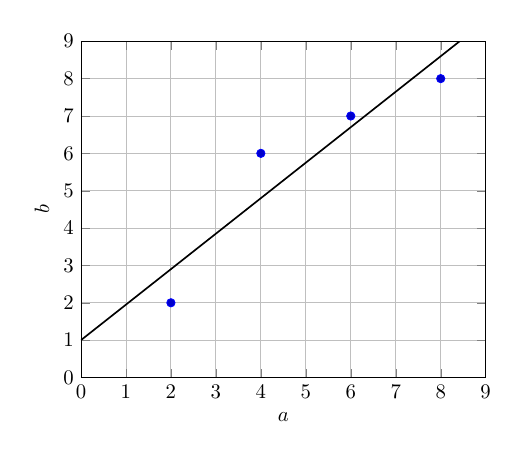
\begin{tikzpicture}[scale=0.75]
\begin{axis}[xlabel=$a$, ylabel=$b$, xmin=0, xmax=9, ymin=0, ymax=9,
             xtick={0,1,...,9}, ytick={0,1,...,9}, grid=major]
  \addplot+[only marks, mark=*] coordinates {(2,2) (4,6) (6,7) (8,8)};
  \addplot[thick, domain=0:9]{0.95 * x + 1};
\end{axis}
\end{tikzpicture}
\end{center}
\end{FigureBlock}
\FigureDescription{Horizontal axis $a$ runs from 0 to 9 with integer ticks;
vertical axis $b$ runs from 0 to 9 with integer ticks. The fitted line is
$b = 0.95a + 1$, passing through 1 at $a=0$ and 9.55 at $a=9$. It lies above
the first measured point and below the third.}

\begin{DataTable}[table/header-rows={1}]
\begin{center}
\begin{tabular}{|c|c|}
\hline
$a$ & $b$ \\
\hline
2 & 2 \\
4 & 6 \\
6 & 7 \\
8 & 8 \\
\hline
\end{tabular}
\end{center}
\end{DataTable}

\questionpart[10]
Set up the normal equations for the least-squares fit and solve for the slope
and intercept.

\begin{solution}
With $\mathbf{A}$ the matrix whose rows are $[a_i \;\; 1]$ and $\vec{b}$ the
vector of measurements, the normal equations are
$\mathbf{A}^{\!\top}\mathbf{A}\,\vec{x} = \mathbf{A}^{\!\top}\vec{b}$, giving a
slope of $0.95$ and an intercept of $1$.
\end{solution}

% ----------------------------------------------------------------------------
\question{Written Response}

\questionpart
State, in one sentence, why the residuals of a least-squares fit must be
orthogonal to the column space of $\mathbf{A}$.

% A tagged answer region, announced as such. The corpus used
% \framebox(470,42){} here, which is picture-mode and carries no semantics.
\answerbox[4\baselineskip]

\end{document}
"
%   pdflatex "\PassOptionsToClass{prob}{latexa11y-assignment}% Demonstration homework, built from real EECS 16A material.
%
% Build both variants from this ONE source. The class option is NOT written
% here, so build.sh can supply it:
%   pdflatex "\PassOptionsToClass{sol}{latexa11y-assignment}\input{demo-homework}"
%   pdflatex "\PassOptionsToClass{prob}{latexa11y-assignment}\input{demo-homework}"
% Hard-coding [sol] below would make `prob` a no-op, because both options would
% be processed and whichever \DeclareOption runs last wins.
%
% Open the result in a PDF reader and look at the bookmark/navigation pane:
% Homework 9 > Question 1 > Part (a) > Solution. Then run a screen reader over
% the figures: each is announced by its description, never by its contents.

\DocumentMetadata{
  lang       = en-US,
  pdfversion = 2.0,
  testphase  = {phase-III,math,table,graphic,firstaid},
}
\documentclass{latexa11y-assignment}

\usepackage{tikz}
\usepackage{pgfplots}
\pgfplotsset{compat=1.16}
\usepackage[american]{circuitikz}

\coursenumber{EECS 16A}
\coursename{Designing Information Devices and Systems I}
\semester{Spring 2026}
\university{UC Berkeley}

\begin{document}

\title{Homework 9}
\maketitle

\noindent
This homework is due Friday, April 3, 2026, at 23:59. Self-grades are due
Monday, April 6, 2026, at 23:59.

% ----------------------------------------------------------------------------
\question{Capacitor Charge Sharing}

Two capacitors are connected through a switch. Before $t=0$ the switch $S_1$ is
open, capacitor $C_1$ is charged to $V_1(0) = 5$\,V, and $C_2$ is uncharged.

% The figure speaks ONLY the description below. The labels drawn inside the
% schematic are never announced.
\begin{AltOnly}{Two capacitors, C1 and C2, each connected from its own top node
to ground, with switch S1 joining the two top nodes. C1 carries voltage V1 and
C2 carries voltage V2, both positive at the top.}
\begin{center}
\begin{circuitikz}[scale=0.9]
  \draw (0, 0) node[ground]{}
    (0, 3) to [C=$C_1$, v=$V_1$] ++ (0, -3)
    (0, 3) to [switch, l=$S_1$] ++ (6, 0)
          to [C=$C_2$, v=$V_2$] ++ (0, -3)
    node[ground]{};
\end{circuitikz}
\end{center}
\end{AltOnly}

\questionpart[5]
Express the total charge stored on both capacitors immediately before the
switch closes.

\begin{solution}
Only $C_1$ is charged, so $Q_{\text{total}} = C_1 V_1(0)$.
\end{solution}

\questionpart[5]
Find the steady-state voltage across both capacitors after the switch closes.

\begin{solution}
Charge is conserved and the two capacitors share a node, so they settle to a
common voltage
\[
  V_\infty = \frac{C_1 V_1(0)}{C_1 + C_2}.
\]
\end{solution}

% ----------------------------------------------------------------------------
\question{Least Squares Fit}

The table below records four measurements. A best-fit line has already been
drawn through them.

% Short /Alt plus a visible long description and a real data table: the tier
% for a figure whose data cannot fit in one spoken sentence.
\begin{FigureBlock}[alt={Scatter plot of b against a on axes running 0 to 9,
with four measured points and a straight best-fit line.}]
\begin{center}
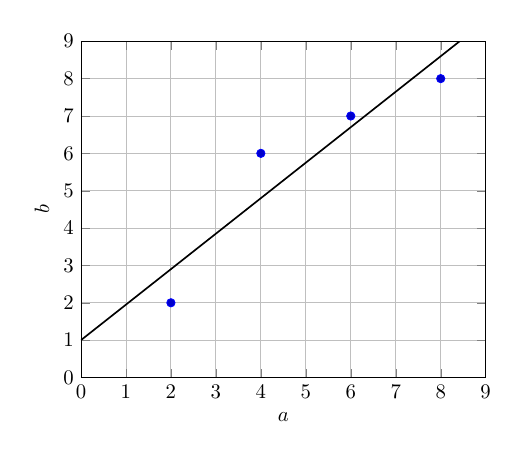
\begin{tikzpicture}[scale=0.75]
\begin{axis}[xlabel=$a$, ylabel=$b$, xmin=0, xmax=9, ymin=0, ymax=9,
             xtick={0,1,...,9}, ytick={0,1,...,9}, grid=major]
  \addplot+[only marks, mark=*] coordinates {(2,2) (4,6) (6,7) (8,8)};
  \addplot[thick, domain=0:9]{0.95 * x + 1};
\end{axis}
\end{tikzpicture}
\end{center}
\end{FigureBlock}
\FigureDescription{Horizontal axis $a$ runs from 0 to 9 with integer ticks;
vertical axis $b$ runs from 0 to 9 with integer ticks. The fitted line is
$b = 0.95a + 1$, passing through 1 at $a=0$ and 9.55 at $a=9$. It lies above
the first measured point and below the third.}

\begin{DataTable}[table/header-rows={1}]
\begin{center}
\begin{tabular}{|c|c|}
\hline
$a$ & $b$ \\
\hline
2 & 2 \\
4 & 6 \\
6 & 7 \\
8 & 8 \\
\hline
\end{tabular}
\end{center}
\end{DataTable}

\questionpart[10]
Set up the normal equations for the least-squares fit and solve for the slope
and intercept.

\begin{solution}
With $\mathbf{A}$ the matrix whose rows are $[a_i \;\; 1]$ and $\vec{b}$ the
vector of measurements, the normal equations are
$\mathbf{A}^{\!\top}\mathbf{A}\,\vec{x} = \mathbf{A}^{\!\top}\vec{b}$, giving a
slope of $0.95$ and an intercept of $1$.
\end{solution}

% ----------------------------------------------------------------------------
\question{Written Response}

\questionpart
State, in one sentence, why the residuals of a least-squares fit must be
orthogonal to the column space of $\mathbf{A}$.

% A tagged answer region, announced as such. The corpus used
% \framebox(470,42){} here, which is picture-mode and carries no semantics.
\answerbox[4\baselineskip]

\end{document}
"
% Hard-coding [sol] below would make `prob` a no-op, because both options would
% be processed and whichever \DeclareOption runs last wins.
%
% Open the result in a PDF reader and look at the bookmark/navigation pane:
% Homework 9 > Question 1 > Part (a) > Solution. Then run a screen reader over
% the figures: each is announced by its description, never by its contents.

\DocumentMetadata{
  lang       = en-US,
  pdfversion = 2.0,
  testphase  = {phase-III,math,table,graphic,firstaid},
}
\documentclass{latexa11y-assignment}

\usepackage{tikz}
\usepackage{pgfplots}
\pgfplotsset{compat=1.16}
\usepackage[american]{circuitikz}

\coursenumber{EECS 16A}
\coursename{Designing Information Devices and Systems I}
\semester{Spring 2026}
\university{UC Berkeley}

\begin{document}

\title{Homework 9}
\maketitle

\noindent
This homework is due Friday, April 3, 2026, at 23:59. Self-grades are due
Monday, April 6, 2026, at 23:59.

% ----------------------------------------------------------------------------
\question{Capacitor Charge Sharing}

Two capacitors are connected through a switch. Before $t=0$ the switch $S_1$ is
open, capacitor $C_1$ is charged to $V_1(0) = 5$\,V, and $C_2$ is uncharged.

% The figure speaks ONLY the description below. The labels drawn inside the
% schematic are never announced.
\begin{AltOnly}{Two capacitors, C1 and C2, each connected from its own top node
to ground, with switch S1 joining the two top nodes. C1 carries voltage V1 and
C2 carries voltage V2, both positive at the top.}
\begin{center}
\begin{circuitikz}[scale=0.9]
  \draw (0, 0) node[ground]{}
    (0, 3) to [C=$C_1$, v=$V_1$] ++ (0, -3)
    (0, 3) to [switch, l=$S_1$] ++ (6, 0)
          to [C=$C_2$, v=$V_2$] ++ (0, -3)
    node[ground]{};
\end{circuitikz}
\end{center}
\end{AltOnly}

\questionpart[5]
Express the total charge stored on both capacitors immediately before the
switch closes.

\begin{solution}
Only $C_1$ is charged, so $Q_{\text{total}} = C_1 V_1(0)$.
\end{solution}

\questionpart[5]
Find the steady-state voltage across both capacitors after the switch closes.

\begin{solution}
Charge is conserved and the two capacitors share a node, so they settle to a
common voltage
\[
  V_\infty = \frac{C_1 V_1(0)}{C_1 + C_2}.
\]
\end{solution}

% ----------------------------------------------------------------------------
\question{Least Squares Fit}

The table below records four measurements. A best-fit line has already been
drawn through them.

% Short /Alt plus a visible long description and a real data table: the tier
% for a figure whose data cannot fit in one spoken sentence.
\begin{FigureBlock}[alt={Scatter plot of b against a on axes running 0 to 9,
with four measured points and a straight best-fit line.}]
\begin{center}
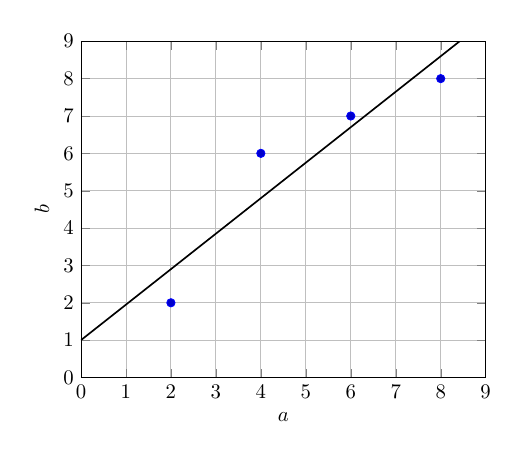
\begin{tikzpicture}[scale=0.75]
\begin{axis}[xlabel=$a$, ylabel=$b$, xmin=0, xmax=9, ymin=0, ymax=9,
             xtick={0,1,...,9}, ytick={0,1,...,9}, grid=major]
  \addplot+[only marks, mark=*] coordinates {(2,2) (4,6) (6,7) (8,8)};
  \addplot[thick, domain=0:9]{0.95 * x + 1};
\end{axis}
\end{tikzpicture}
\end{center}
\end{FigureBlock}
\FigureDescription{Horizontal axis $a$ runs from 0 to 9 with integer ticks;
vertical axis $b$ runs from 0 to 9 with integer ticks. The fitted line is
$b = 0.95a + 1$, passing through 1 at $a=0$ and 9.55 at $a=9$. It lies above
the first measured point and below the third.}

\begin{DataTable}[table/header-rows={1}]
\begin{center}
\begin{tabular}{|c|c|}
\hline
$a$ & $b$ \\
\hline
2 & 2 \\
4 & 6 \\
6 & 7 \\
8 & 8 \\
\hline
\end{tabular}
\end{center}
\end{DataTable}

\questionpart[10]
Set up the normal equations for the least-squares fit and solve for the slope
and intercept.

\begin{solution}
With $\mathbf{A}$ the matrix whose rows are $[a_i \;\; 1]$ and $\vec{b}$ the
vector of measurements, the normal equations are
$\mathbf{A}^{\!\top}\mathbf{A}\,\vec{x} = \mathbf{A}^{\!\top}\vec{b}$, giving a
slope of $0.95$ and an intercept of $1$.
\end{solution}

% ----------------------------------------------------------------------------
\question{Written Response}

\questionpart
State, in one sentence, why the residuals of a least-squares fit must be
orthogonal to the column space of $\mathbf{A}$.

% A tagged answer region, announced as such. The corpus used
% \framebox(470,42){} here, which is picture-mode and carries no semantics.
\answerbox[4\baselineskip]

\end{document}
"
% Hard-coding [sol] below would make `prob` a no-op, because both options would
% be processed and whichever \DeclareOption runs last wins.
%
% Open the result in a PDF reader and look at the bookmark/navigation pane:
% Homework 9 > Question 1 > Part (a) > Solution. Then run a screen reader over
% the figures: each is announced by its description, never by its contents.

\DocumentMetadata{
  lang       = en-US,
  pdfversion = 2.0,
  testphase  = {phase-III,math,table,graphic,firstaid},
}
\documentclass{latexa11y-assignment}

\usepackage{tikz}
\usepackage{pgfplots}
\pgfplotsset{compat=1.16}
\usepackage[american]{circuitikz}

\coursenumber{EECS 16A}
\coursename{Designing Information Devices and Systems I}
\semester{Spring 2026}
\university{UC Berkeley}

\begin{document}

\title{Homework 9}
\maketitle

\noindent
This homework is due Friday, April 3, 2026, at 23:59. Self-grades are due
Monday, April 6, 2026, at 23:59.

% ----------------------------------------------------------------------------
\question{Capacitor Charge Sharing}

Two capacitors are connected through a switch. Before $t=0$ the switch $S_1$ is
open, capacitor $C_1$ is charged to $V_1(0) = 5$\,V, and $C_2$ is uncharged.

% The figure speaks ONLY the description below. The labels drawn inside the
% schematic are never announced.
\begin{AltOnly}{Two capacitors, C1 and C2, each connected from its own top node
to ground, with switch S1 joining the two top nodes. C1 carries voltage V1 and
C2 carries voltage V2, both positive at the top.}
\begin{center}
\begin{circuitikz}[scale=0.9]
  \draw (0, 0) node[ground]{}
    (0, 3) to [C=$C_1$, v=$V_1$] ++ (0, -3)
    (0, 3) to [switch, l=$S_1$] ++ (6, 0)
          to [C=$C_2$, v=$V_2$] ++ (0, -3)
    node[ground]{};
\end{circuitikz}
\end{center}
\end{AltOnly}

\questionpart[5]
Express the total charge stored on both capacitors immediately before the
switch closes.

\begin{solution}
Only $C_1$ is charged, so $Q_{\text{total}} = C_1 V_1(0)$.
\end{solution}

\questionpart[5]
Find the steady-state voltage across both capacitors after the switch closes.

\begin{solution}
Charge is conserved and the two capacitors share a node, so they settle to a
common voltage
\[
  V_\infty = \frac{C_1 V_1(0)}{C_1 + C_2}.
\]
\end{solution}

% ----------------------------------------------------------------------------
\question{Least Squares Fit}

The table below records four measurements. A best-fit line has already been
drawn through them.

% Short /Alt plus a visible long description and a real data table: the tier
% for a figure whose data cannot fit in one spoken sentence.
\begin{FigureBlock}[alt={Scatter plot of b against a on axes running 0 to 9,
with four measured points and a straight best-fit line.}]
\begin{center}
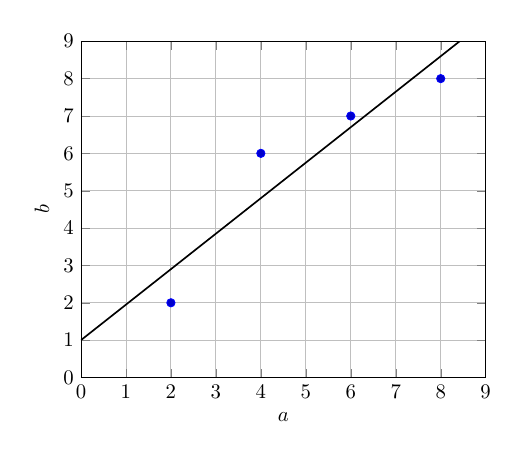
\begin{tikzpicture}[scale=0.75]
\begin{axis}[xlabel=$a$, ylabel=$b$, xmin=0, xmax=9, ymin=0, ymax=9,
             xtick={0,1,...,9}, ytick={0,1,...,9}, grid=major]
  \addplot+[only marks, mark=*] coordinates {(2,2) (4,6) (6,7) (8,8)};
  \addplot[thick, domain=0:9]{0.95 * x + 1};
\end{axis}
\end{tikzpicture}
\end{center}
\end{FigureBlock}
\FigureDescription{Horizontal axis $a$ runs from 0 to 9 with integer ticks;
vertical axis $b$ runs from 0 to 9 with integer ticks. The fitted line is
$b = 0.95a + 1$, passing through 1 at $a=0$ and 9.55 at $a=9$. It lies above
the first measured point and below the third.}

\begin{DataTable}[table/header-rows={1}]
\begin{center}
\begin{tabular}{|c|c|}
\hline
$a$ & $b$ \\
\hline
2 & 2 \\
4 & 6 \\
6 & 7 \\
8 & 8 \\
\hline
\end{tabular}
\end{center}
\end{DataTable}

\questionpart[10]
Set up the normal equations for the least-squares fit and solve for the slope
and intercept.

\begin{solution}
With $\mathbf{A}$ the matrix whose rows are $[a_i \;\; 1]$ and $\vec{b}$ the
vector of measurements, the normal equations are
$\mathbf{A}^{\!\top}\mathbf{A}\,\vec{x} = \mathbf{A}^{\!\top}\vec{b}$, giving a
slope of $0.95$ and an intercept of $1$.
\end{solution}

% ----------------------------------------------------------------------------
\question{Written Response}

\questionpart
State, in one sentence, why the residuals of a least-squares fit must be
orthogonal to the column space of $\mathbf{A}$.

% A tagged answer region, announced as such. The corpus used
% \framebox(470,42){} here, which is picture-mode and carries no semantics.
\answerbox[4\baselineskip]

\end{document}
"
%   pdflatex "\PassOptionsToClass{prob}{latexa11y-assignment}% Demonstration homework, built from real EECS 16A material.
%
% Build both variants from this ONE source. The class option is NOT written
% here, so build.sh can supply it:
%   pdflatex "\PassOptionsToClass{sol}{latexa11y-assignment}% Demonstration homework, built from real EECS 16A material.
%
% Build both variants from this ONE source. The class option is NOT written
% here, so build.sh can supply it:
%   pdflatex "\PassOptionsToClass{sol}{latexa11y-assignment}% Demonstration homework, built from real EECS 16A material.
%
% Build both variants from this ONE source. The class option is NOT written
% here, so build.sh can supply it:
%   pdflatex "\PassOptionsToClass{sol}{latexa11y-assignment}\input{demo-homework}"
%   pdflatex "\PassOptionsToClass{prob}{latexa11y-assignment}\input{demo-homework}"
% Hard-coding [sol] below would make `prob` a no-op, because both options would
% be processed and whichever \DeclareOption runs last wins.
%
% Open the result in a PDF reader and look at the bookmark/navigation pane:
% Homework 9 > Question 1 > Part (a) > Solution. Then run a screen reader over
% the figures: each is announced by its description, never by its contents.

\DocumentMetadata{
  lang       = en-US,
  pdfversion = 2.0,
  testphase  = {phase-III,math,table,graphic,firstaid},
}
\documentclass{latexa11y-assignment}

\usepackage{tikz}
\usepackage{pgfplots}
\pgfplotsset{compat=1.16}
\usepackage[american]{circuitikz}

\coursenumber{EECS 16A}
\coursename{Designing Information Devices and Systems I}
\semester{Spring 2026}
\university{UC Berkeley}

\begin{document}

\title{Homework 9}
\maketitle

\noindent
This homework is due Friday, April 3, 2026, at 23:59. Self-grades are due
Monday, April 6, 2026, at 23:59.

% ----------------------------------------------------------------------------
\question{Capacitor Charge Sharing}

Two capacitors are connected through a switch. Before $t=0$ the switch $S_1$ is
open, capacitor $C_1$ is charged to $V_1(0) = 5$\,V, and $C_2$ is uncharged.

% The figure speaks ONLY the description below. The labels drawn inside the
% schematic are never announced.
\begin{AltOnly}{Two capacitors, C1 and C2, each connected from its own top node
to ground, with switch S1 joining the two top nodes. C1 carries voltage V1 and
C2 carries voltage V2, both positive at the top.}
\begin{center}
\begin{circuitikz}[scale=0.9]
  \draw (0, 0) node[ground]{}
    (0, 3) to [C=$C_1$, v=$V_1$] ++ (0, -3)
    (0, 3) to [switch, l=$S_1$] ++ (6, 0)
          to [C=$C_2$, v=$V_2$] ++ (0, -3)
    node[ground]{};
\end{circuitikz}
\end{center}
\end{AltOnly}

\questionpart[5]
Express the total charge stored on both capacitors immediately before the
switch closes.

\begin{solution}
Only $C_1$ is charged, so $Q_{\text{total}} = C_1 V_1(0)$.
\end{solution}

\questionpart[5]
Find the steady-state voltage across both capacitors after the switch closes.

\begin{solution}
Charge is conserved and the two capacitors share a node, so they settle to a
common voltage
\[
  V_\infty = \frac{C_1 V_1(0)}{C_1 + C_2}.
\]
\end{solution}

% ----------------------------------------------------------------------------
\question{Least Squares Fit}

The table below records four measurements. A best-fit line has already been
drawn through them.

% Short /Alt plus a visible long description and a real data table: the tier
% for a figure whose data cannot fit in one spoken sentence.
\begin{FigureBlock}[alt={Scatter plot of b against a on axes running 0 to 9,
with four measured points and a straight best-fit line.}]
\begin{center}
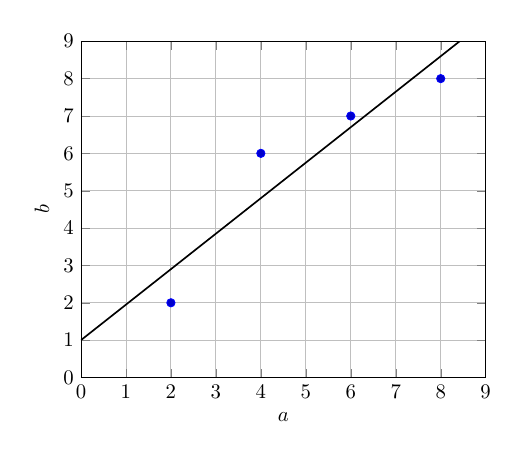
\begin{tikzpicture}[scale=0.75]
\begin{axis}[xlabel=$a$, ylabel=$b$, xmin=0, xmax=9, ymin=0, ymax=9,
             xtick={0,1,...,9}, ytick={0,1,...,9}, grid=major]
  \addplot+[only marks, mark=*] coordinates {(2,2) (4,6) (6,7) (8,8)};
  \addplot[thick, domain=0:9]{0.95 * x + 1};
\end{axis}
\end{tikzpicture}
\end{center}
\end{FigureBlock}
\FigureDescription{Horizontal axis $a$ runs from 0 to 9 with integer ticks;
vertical axis $b$ runs from 0 to 9 with integer ticks. The fitted line is
$b = 0.95a + 1$, passing through 1 at $a=0$ and 9.55 at $a=9$. It lies above
the first measured point and below the third.}

\begin{DataTable}[table/header-rows={1}]
\begin{center}
\begin{tabular}{|c|c|}
\hline
$a$ & $b$ \\
\hline
2 & 2 \\
4 & 6 \\
6 & 7 \\
8 & 8 \\
\hline
\end{tabular}
\end{center}
\end{DataTable}

\questionpart[10]
Set up the normal equations for the least-squares fit and solve for the slope
and intercept.

\begin{solution}
With $\mathbf{A}$ the matrix whose rows are $[a_i \;\; 1]$ and $\vec{b}$ the
vector of measurements, the normal equations are
$\mathbf{A}^{\!\top}\mathbf{A}\,\vec{x} = \mathbf{A}^{\!\top}\vec{b}$, giving a
slope of $0.95$ and an intercept of $1$.
\end{solution}

% ----------------------------------------------------------------------------
\question{Written Response}

\questionpart
State, in one sentence, why the residuals of a least-squares fit must be
orthogonal to the column space of $\mathbf{A}$.

% A tagged answer region, announced as such. The corpus used
% \framebox(470,42){} here, which is picture-mode and carries no semantics.
\answerbox[4\baselineskip]

\end{document}
"
%   pdflatex "\PassOptionsToClass{prob}{latexa11y-assignment}% Demonstration homework, built from real EECS 16A material.
%
% Build both variants from this ONE source. The class option is NOT written
% here, so build.sh can supply it:
%   pdflatex "\PassOptionsToClass{sol}{latexa11y-assignment}\input{demo-homework}"
%   pdflatex "\PassOptionsToClass{prob}{latexa11y-assignment}\input{demo-homework}"
% Hard-coding [sol] below would make `prob` a no-op, because both options would
% be processed and whichever \DeclareOption runs last wins.
%
% Open the result in a PDF reader and look at the bookmark/navigation pane:
% Homework 9 > Question 1 > Part (a) > Solution. Then run a screen reader over
% the figures: each is announced by its description, never by its contents.

\DocumentMetadata{
  lang       = en-US,
  pdfversion = 2.0,
  testphase  = {phase-III,math,table,graphic,firstaid},
}
\documentclass{latexa11y-assignment}

\usepackage{tikz}
\usepackage{pgfplots}
\pgfplotsset{compat=1.16}
\usepackage[american]{circuitikz}

\coursenumber{EECS 16A}
\coursename{Designing Information Devices and Systems I}
\semester{Spring 2026}
\university{UC Berkeley}

\begin{document}

\title{Homework 9}
\maketitle

\noindent
This homework is due Friday, April 3, 2026, at 23:59. Self-grades are due
Monday, April 6, 2026, at 23:59.

% ----------------------------------------------------------------------------
\question{Capacitor Charge Sharing}

Two capacitors are connected through a switch. Before $t=0$ the switch $S_1$ is
open, capacitor $C_1$ is charged to $V_1(0) = 5$\,V, and $C_2$ is uncharged.

% The figure speaks ONLY the description below. The labels drawn inside the
% schematic are never announced.
\begin{AltOnly}{Two capacitors, C1 and C2, each connected from its own top node
to ground, with switch S1 joining the two top nodes. C1 carries voltage V1 and
C2 carries voltage V2, both positive at the top.}
\begin{center}
\begin{circuitikz}[scale=0.9]
  \draw (0, 0) node[ground]{}
    (0, 3) to [C=$C_1$, v=$V_1$] ++ (0, -3)
    (0, 3) to [switch, l=$S_1$] ++ (6, 0)
          to [C=$C_2$, v=$V_2$] ++ (0, -3)
    node[ground]{};
\end{circuitikz}
\end{center}
\end{AltOnly}

\questionpart[5]
Express the total charge stored on both capacitors immediately before the
switch closes.

\begin{solution}
Only $C_1$ is charged, so $Q_{\text{total}} = C_1 V_1(0)$.
\end{solution}

\questionpart[5]
Find the steady-state voltage across both capacitors after the switch closes.

\begin{solution}
Charge is conserved and the two capacitors share a node, so they settle to a
common voltage
\[
  V_\infty = \frac{C_1 V_1(0)}{C_1 + C_2}.
\]
\end{solution}

% ----------------------------------------------------------------------------
\question{Least Squares Fit}

The table below records four measurements. A best-fit line has already been
drawn through them.

% Short /Alt plus a visible long description and a real data table: the tier
% for a figure whose data cannot fit in one spoken sentence.
\begin{FigureBlock}[alt={Scatter plot of b against a on axes running 0 to 9,
with four measured points and a straight best-fit line.}]
\begin{center}
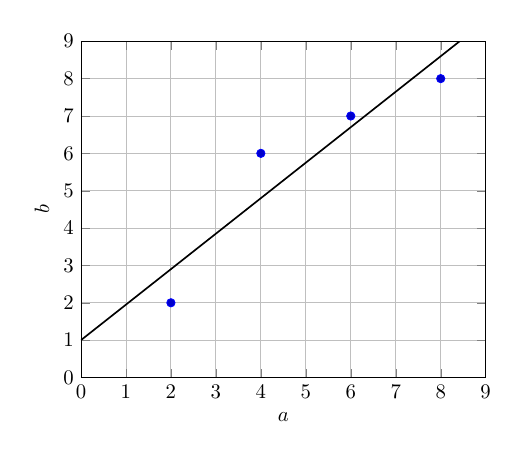
\begin{tikzpicture}[scale=0.75]
\begin{axis}[xlabel=$a$, ylabel=$b$, xmin=0, xmax=9, ymin=0, ymax=9,
             xtick={0,1,...,9}, ytick={0,1,...,9}, grid=major]
  \addplot+[only marks, mark=*] coordinates {(2,2) (4,6) (6,7) (8,8)};
  \addplot[thick, domain=0:9]{0.95 * x + 1};
\end{axis}
\end{tikzpicture}
\end{center}
\end{FigureBlock}
\FigureDescription{Horizontal axis $a$ runs from 0 to 9 with integer ticks;
vertical axis $b$ runs from 0 to 9 with integer ticks. The fitted line is
$b = 0.95a + 1$, passing through 1 at $a=0$ and 9.55 at $a=9$. It lies above
the first measured point and below the third.}

\begin{DataTable}[table/header-rows={1}]
\begin{center}
\begin{tabular}{|c|c|}
\hline
$a$ & $b$ \\
\hline
2 & 2 \\
4 & 6 \\
6 & 7 \\
8 & 8 \\
\hline
\end{tabular}
\end{center}
\end{DataTable}

\questionpart[10]
Set up the normal equations for the least-squares fit and solve for the slope
and intercept.

\begin{solution}
With $\mathbf{A}$ the matrix whose rows are $[a_i \;\; 1]$ and $\vec{b}$ the
vector of measurements, the normal equations are
$\mathbf{A}^{\!\top}\mathbf{A}\,\vec{x} = \mathbf{A}^{\!\top}\vec{b}$, giving a
slope of $0.95$ and an intercept of $1$.
\end{solution}

% ----------------------------------------------------------------------------
\question{Written Response}

\questionpart
State, in one sentence, why the residuals of a least-squares fit must be
orthogonal to the column space of $\mathbf{A}$.

% A tagged answer region, announced as such. The corpus used
% \framebox(470,42){} here, which is picture-mode and carries no semantics.
\answerbox[4\baselineskip]

\end{document}
"
% Hard-coding [sol] below would make `prob` a no-op, because both options would
% be processed and whichever \DeclareOption runs last wins.
%
% Open the result in a PDF reader and look at the bookmark/navigation pane:
% Homework 9 > Question 1 > Part (a) > Solution. Then run a screen reader over
% the figures: each is announced by its description, never by its contents.

\DocumentMetadata{
  lang       = en-US,
  pdfversion = 2.0,
  testphase  = {phase-III,math,table,graphic,firstaid},
}
\documentclass{latexa11y-assignment}

\usepackage{tikz}
\usepackage{pgfplots}
\pgfplotsset{compat=1.16}
\usepackage[american]{circuitikz}

\coursenumber{EECS 16A}
\coursename{Designing Information Devices and Systems I}
\semester{Spring 2026}
\university{UC Berkeley}

\begin{document}

\title{Homework 9}
\maketitle

\noindent
This homework is due Friday, April 3, 2026, at 23:59. Self-grades are due
Monday, April 6, 2026, at 23:59.

% ----------------------------------------------------------------------------
\question{Capacitor Charge Sharing}

Two capacitors are connected through a switch. Before $t=0$ the switch $S_1$ is
open, capacitor $C_1$ is charged to $V_1(0) = 5$\,V, and $C_2$ is uncharged.

% The figure speaks ONLY the description below. The labels drawn inside the
% schematic are never announced.
\begin{AltOnly}{Two capacitors, C1 and C2, each connected from its own top node
to ground, with switch S1 joining the two top nodes. C1 carries voltage V1 and
C2 carries voltage V2, both positive at the top.}
\begin{center}
\begin{circuitikz}[scale=0.9]
  \draw (0, 0) node[ground]{}
    (0, 3) to [C=$C_1$, v=$V_1$] ++ (0, -3)
    (0, 3) to [switch, l=$S_1$] ++ (6, 0)
          to [C=$C_2$, v=$V_2$] ++ (0, -3)
    node[ground]{};
\end{circuitikz}
\end{center}
\end{AltOnly}

\questionpart[5]
Express the total charge stored on both capacitors immediately before the
switch closes.

\begin{solution}
Only $C_1$ is charged, so $Q_{\text{total}} = C_1 V_1(0)$.
\end{solution}

\questionpart[5]
Find the steady-state voltage across both capacitors after the switch closes.

\begin{solution}
Charge is conserved and the two capacitors share a node, so they settle to a
common voltage
\[
  V_\infty = \frac{C_1 V_1(0)}{C_1 + C_2}.
\]
\end{solution}

% ----------------------------------------------------------------------------
\question{Least Squares Fit}

The table below records four measurements. A best-fit line has already been
drawn through them.

% Short /Alt plus a visible long description and a real data table: the tier
% for a figure whose data cannot fit in one spoken sentence.
\begin{FigureBlock}[alt={Scatter plot of b against a on axes running 0 to 9,
with four measured points and a straight best-fit line.}]
\begin{center}
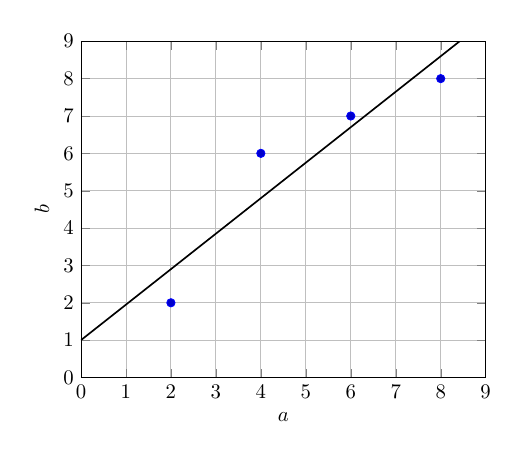
\begin{tikzpicture}[scale=0.75]
\begin{axis}[xlabel=$a$, ylabel=$b$, xmin=0, xmax=9, ymin=0, ymax=9,
             xtick={0,1,...,9}, ytick={0,1,...,9}, grid=major]
  \addplot+[only marks, mark=*] coordinates {(2,2) (4,6) (6,7) (8,8)};
  \addplot[thick, domain=0:9]{0.95 * x + 1};
\end{axis}
\end{tikzpicture}
\end{center}
\end{FigureBlock}
\FigureDescription{Horizontal axis $a$ runs from 0 to 9 with integer ticks;
vertical axis $b$ runs from 0 to 9 with integer ticks. The fitted line is
$b = 0.95a + 1$, passing through 1 at $a=0$ and 9.55 at $a=9$. It lies above
the first measured point and below the third.}

\begin{DataTable}[table/header-rows={1}]
\begin{center}
\begin{tabular}{|c|c|}
\hline
$a$ & $b$ \\
\hline
2 & 2 \\
4 & 6 \\
6 & 7 \\
8 & 8 \\
\hline
\end{tabular}
\end{center}
\end{DataTable}

\questionpart[10]
Set up the normal equations for the least-squares fit and solve for the slope
and intercept.

\begin{solution}
With $\mathbf{A}$ the matrix whose rows are $[a_i \;\; 1]$ and $\vec{b}$ the
vector of measurements, the normal equations are
$\mathbf{A}^{\!\top}\mathbf{A}\,\vec{x} = \mathbf{A}^{\!\top}\vec{b}$, giving a
slope of $0.95$ and an intercept of $1$.
\end{solution}

% ----------------------------------------------------------------------------
\question{Written Response}

\questionpart
State, in one sentence, why the residuals of a least-squares fit must be
orthogonal to the column space of $\mathbf{A}$.

% A tagged answer region, announced as such. The corpus used
% \framebox(470,42){} here, which is picture-mode and carries no semantics.
\answerbox[4\baselineskip]

\end{document}
"
%   pdflatex "\PassOptionsToClass{prob}{latexa11y-assignment}% Demonstration homework, built from real EECS 16A material.
%
% Build both variants from this ONE source. The class option is NOT written
% here, so build.sh can supply it:
%   pdflatex "\PassOptionsToClass{sol}{latexa11y-assignment}% Demonstration homework, built from real EECS 16A material.
%
% Build both variants from this ONE source. The class option is NOT written
% here, so build.sh can supply it:
%   pdflatex "\PassOptionsToClass{sol}{latexa11y-assignment}\input{demo-homework}"
%   pdflatex "\PassOptionsToClass{prob}{latexa11y-assignment}\input{demo-homework}"
% Hard-coding [sol] below would make `prob` a no-op, because both options would
% be processed and whichever \DeclareOption runs last wins.
%
% Open the result in a PDF reader and look at the bookmark/navigation pane:
% Homework 9 > Question 1 > Part (a) > Solution. Then run a screen reader over
% the figures: each is announced by its description, never by its contents.

\DocumentMetadata{
  lang       = en-US,
  pdfversion = 2.0,
  testphase  = {phase-III,math,table,graphic,firstaid},
}
\documentclass{latexa11y-assignment}

\usepackage{tikz}
\usepackage{pgfplots}
\pgfplotsset{compat=1.16}
\usepackage[american]{circuitikz}

\coursenumber{EECS 16A}
\coursename{Designing Information Devices and Systems I}
\semester{Spring 2026}
\university{UC Berkeley}

\begin{document}

\title{Homework 9}
\maketitle

\noindent
This homework is due Friday, April 3, 2026, at 23:59. Self-grades are due
Monday, April 6, 2026, at 23:59.

% ----------------------------------------------------------------------------
\question{Capacitor Charge Sharing}

Two capacitors are connected through a switch. Before $t=0$ the switch $S_1$ is
open, capacitor $C_1$ is charged to $V_1(0) = 5$\,V, and $C_2$ is uncharged.

% The figure speaks ONLY the description below. The labels drawn inside the
% schematic are never announced.
\begin{AltOnly}{Two capacitors, C1 and C2, each connected from its own top node
to ground, with switch S1 joining the two top nodes. C1 carries voltage V1 and
C2 carries voltage V2, both positive at the top.}
\begin{center}
\begin{circuitikz}[scale=0.9]
  \draw (0, 0) node[ground]{}
    (0, 3) to [C=$C_1$, v=$V_1$] ++ (0, -3)
    (0, 3) to [switch, l=$S_1$] ++ (6, 0)
          to [C=$C_2$, v=$V_2$] ++ (0, -3)
    node[ground]{};
\end{circuitikz}
\end{center}
\end{AltOnly}

\questionpart[5]
Express the total charge stored on both capacitors immediately before the
switch closes.

\begin{solution}
Only $C_1$ is charged, so $Q_{\text{total}} = C_1 V_1(0)$.
\end{solution}

\questionpart[5]
Find the steady-state voltage across both capacitors after the switch closes.

\begin{solution}
Charge is conserved and the two capacitors share a node, so they settle to a
common voltage
\[
  V_\infty = \frac{C_1 V_1(0)}{C_1 + C_2}.
\]
\end{solution}

% ----------------------------------------------------------------------------
\question{Least Squares Fit}

The table below records four measurements. A best-fit line has already been
drawn through them.

% Short /Alt plus a visible long description and a real data table: the tier
% for a figure whose data cannot fit in one spoken sentence.
\begin{FigureBlock}[alt={Scatter plot of b against a on axes running 0 to 9,
with four measured points and a straight best-fit line.}]
\begin{center}
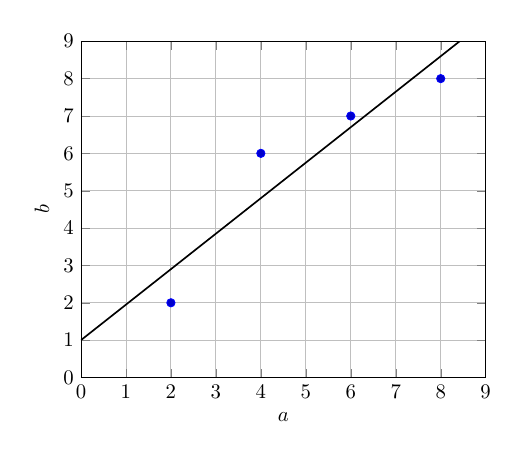
\begin{tikzpicture}[scale=0.75]
\begin{axis}[xlabel=$a$, ylabel=$b$, xmin=0, xmax=9, ymin=0, ymax=9,
             xtick={0,1,...,9}, ytick={0,1,...,9}, grid=major]
  \addplot+[only marks, mark=*] coordinates {(2,2) (4,6) (6,7) (8,8)};
  \addplot[thick, domain=0:9]{0.95 * x + 1};
\end{axis}
\end{tikzpicture}
\end{center}
\end{FigureBlock}
\FigureDescription{Horizontal axis $a$ runs from 0 to 9 with integer ticks;
vertical axis $b$ runs from 0 to 9 with integer ticks. The fitted line is
$b = 0.95a + 1$, passing through 1 at $a=0$ and 9.55 at $a=9$. It lies above
the first measured point and below the third.}

\begin{DataTable}[table/header-rows={1}]
\begin{center}
\begin{tabular}{|c|c|}
\hline
$a$ & $b$ \\
\hline
2 & 2 \\
4 & 6 \\
6 & 7 \\
8 & 8 \\
\hline
\end{tabular}
\end{center}
\end{DataTable}

\questionpart[10]
Set up the normal equations for the least-squares fit and solve for the slope
and intercept.

\begin{solution}
With $\mathbf{A}$ the matrix whose rows are $[a_i \;\; 1]$ and $\vec{b}$ the
vector of measurements, the normal equations are
$\mathbf{A}^{\!\top}\mathbf{A}\,\vec{x} = \mathbf{A}^{\!\top}\vec{b}$, giving a
slope of $0.95$ and an intercept of $1$.
\end{solution}

% ----------------------------------------------------------------------------
\question{Written Response}

\questionpart
State, in one sentence, why the residuals of a least-squares fit must be
orthogonal to the column space of $\mathbf{A}$.

% A tagged answer region, announced as such. The corpus used
% \framebox(470,42){} here, which is picture-mode and carries no semantics.
\answerbox[4\baselineskip]

\end{document}
"
%   pdflatex "\PassOptionsToClass{prob}{latexa11y-assignment}% Demonstration homework, built from real EECS 16A material.
%
% Build both variants from this ONE source. The class option is NOT written
% here, so build.sh can supply it:
%   pdflatex "\PassOptionsToClass{sol}{latexa11y-assignment}\input{demo-homework}"
%   pdflatex "\PassOptionsToClass{prob}{latexa11y-assignment}\input{demo-homework}"
% Hard-coding [sol] below would make `prob` a no-op, because both options would
% be processed and whichever \DeclareOption runs last wins.
%
% Open the result in a PDF reader and look at the bookmark/navigation pane:
% Homework 9 > Question 1 > Part (a) > Solution. Then run a screen reader over
% the figures: each is announced by its description, never by its contents.

\DocumentMetadata{
  lang       = en-US,
  pdfversion = 2.0,
  testphase  = {phase-III,math,table,graphic,firstaid},
}
\documentclass{latexa11y-assignment}

\usepackage{tikz}
\usepackage{pgfplots}
\pgfplotsset{compat=1.16}
\usepackage[american]{circuitikz}

\coursenumber{EECS 16A}
\coursename{Designing Information Devices and Systems I}
\semester{Spring 2026}
\university{UC Berkeley}

\begin{document}

\title{Homework 9}
\maketitle

\noindent
This homework is due Friday, April 3, 2026, at 23:59. Self-grades are due
Monday, April 6, 2026, at 23:59.

% ----------------------------------------------------------------------------
\question{Capacitor Charge Sharing}

Two capacitors are connected through a switch. Before $t=0$ the switch $S_1$ is
open, capacitor $C_1$ is charged to $V_1(0) = 5$\,V, and $C_2$ is uncharged.

% The figure speaks ONLY the description below. The labels drawn inside the
% schematic are never announced.
\begin{AltOnly}{Two capacitors, C1 and C2, each connected from its own top node
to ground, with switch S1 joining the two top nodes. C1 carries voltage V1 and
C2 carries voltage V2, both positive at the top.}
\begin{center}
\begin{circuitikz}[scale=0.9]
  \draw (0, 0) node[ground]{}
    (0, 3) to [C=$C_1$, v=$V_1$] ++ (0, -3)
    (0, 3) to [switch, l=$S_1$] ++ (6, 0)
          to [C=$C_2$, v=$V_2$] ++ (0, -3)
    node[ground]{};
\end{circuitikz}
\end{center}
\end{AltOnly}

\questionpart[5]
Express the total charge stored on both capacitors immediately before the
switch closes.

\begin{solution}
Only $C_1$ is charged, so $Q_{\text{total}} = C_1 V_1(0)$.
\end{solution}

\questionpart[5]
Find the steady-state voltage across both capacitors after the switch closes.

\begin{solution}
Charge is conserved and the two capacitors share a node, so they settle to a
common voltage
\[
  V_\infty = \frac{C_1 V_1(0)}{C_1 + C_2}.
\]
\end{solution}

% ----------------------------------------------------------------------------
\question{Least Squares Fit}

The table below records four measurements. A best-fit line has already been
drawn through them.

% Short /Alt plus a visible long description and a real data table: the tier
% for a figure whose data cannot fit in one spoken sentence.
\begin{FigureBlock}[alt={Scatter plot of b against a on axes running 0 to 9,
with four measured points and a straight best-fit line.}]
\begin{center}
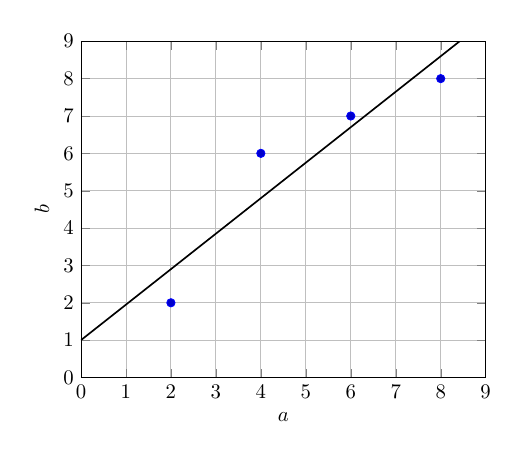
\begin{tikzpicture}[scale=0.75]
\begin{axis}[xlabel=$a$, ylabel=$b$, xmin=0, xmax=9, ymin=0, ymax=9,
             xtick={0,1,...,9}, ytick={0,1,...,9}, grid=major]
  \addplot+[only marks, mark=*] coordinates {(2,2) (4,6) (6,7) (8,8)};
  \addplot[thick, domain=0:9]{0.95 * x + 1};
\end{axis}
\end{tikzpicture}
\end{center}
\end{FigureBlock}
\FigureDescription{Horizontal axis $a$ runs from 0 to 9 with integer ticks;
vertical axis $b$ runs from 0 to 9 with integer ticks. The fitted line is
$b = 0.95a + 1$, passing through 1 at $a=0$ and 9.55 at $a=9$. It lies above
the first measured point and below the third.}

\begin{DataTable}[table/header-rows={1}]
\begin{center}
\begin{tabular}{|c|c|}
\hline
$a$ & $b$ \\
\hline
2 & 2 \\
4 & 6 \\
6 & 7 \\
8 & 8 \\
\hline
\end{tabular}
\end{center}
\end{DataTable}

\questionpart[10]
Set up the normal equations for the least-squares fit and solve for the slope
and intercept.

\begin{solution}
With $\mathbf{A}$ the matrix whose rows are $[a_i \;\; 1]$ and $\vec{b}$ the
vector of measurements, the normal equations are
$\mathbf{A}^{\!\top}\mathbf{A}\,\vec{x} = \mathbf{A}^{\!\top}\vec{b}$, giving a
slope of $0.95$ and an intercept of $1$.
\end{solution}

% ----------------------------------------------------------------------------
\question{Written Response}

\questionpart
State, in one sentence, why the residuals of a least-squares fit must be
orthogonal to the column space of $\mathbf{A}$.

% A tagged answer region, announced as such. The corpus used
% \framebox(470,42){} here, which is picture-mode and carries no semantics.
\answerbox[4\baselineskip]

\end{document}
"
% Hard-coding [sol] below would make `prob` a no-op, because both options would
% be processed and whichever \DeclareOption runs last wins.
%
% Open the result in a PDF reader and look at the bookmark/navigation pane:
% Homework 9 > Question 1 > Part (a) > Solution. Then run a screen reader over
% the figures: each is announced by its description, never by its contents.

\DocumentMetadata{
  lang       = en-US,
  pdfversion = 2.0,
  testphase  = {phase-III,math,table,graphic,firstaid},
}
\documentclass{latexa11y-assignment}

\usepackage{tikz}
\usepackage{pgfplots}
\pgfplotsset{compat=1.16}
\usepackage[american]{circuitikz}

\coursenumber{EECS 16A}
\coursename{Designing Information Devices and Systems I}
\semester{Spring 2026}
\university{UC Berkeley}

\begin{document}

\title{Homework 9}
\maketitle

\noindent
This homework is due Friday, April 3, 2026, at 23:59. Self-grades are due
Monday, April 6, 2026, at 23:59.

% ----------------------------------------------------------------------------
\question{Capacitor Charge Sharing}

Two capacitors are connected through a switch. Before $t=0$ the switch $S_1$ is
open, capacitor $C_1$ is charged to $V_1(0) = 5$\,V, and $C_2$ is uncharged.

% The figure speaks ONLY the description below. The labels drawn inside the
% schematic are never announced.
\begin{AltOnly}{Two capacitors, C1 and C2, each connected from its own top node
to ground, with switch S1 joining the two top nodes. C1 carries voltage V1 and
C2 carries voltage V2, both positive at the top.}
\begin{center}
\begin{circuitikz}[scale=0.9]
  \draw (0, 0) node[ground]{}
    (0, 3) to [C=$C_1$, v=$V_1$] ++ (0, -3)
    (0, 3) to [switch, l=$S_1$] ++ (6, 0)
          to [C=$C_2$, v=$V_2$] ++ (0, -3)
    node[ground]{};
\end{circuitikz}
\end{center}
\end{AltOnly}

\questionpart[5]
Express the total charge stored on both capacitors immediately before the
switch closes.

\begin{solution}
Only $C_1$ is charged, so $Q_{\text{total}} = C_1 V_1(0)$.
\end{solution}

\questionpart[5]
Find the steady-state voltage across both capacitors after the switch closes.

\begin{solution}
Charge is conserved and the two capacitors share a node, so they settle to a
common voltage
\[
  V_\infty = \frac{C_1 V_1(0)}{C_1 + C_2}.
\]
\end{solution}

% ----------------------------------------------------------------------------
\question{Least Squares Fit}

The table below records four measurements. A best-fit line has already been
drawn through them.

% Short /Alt plus a visible long description and a real data table: the tier
% for a figure whose data cannot fit in one spoken sentence.
\begin{FigureBlock}[alt={Scatter plot of b against a on axes running 0 to 9,
with four measured points and a straight best-fit line.}]
\begin{center}
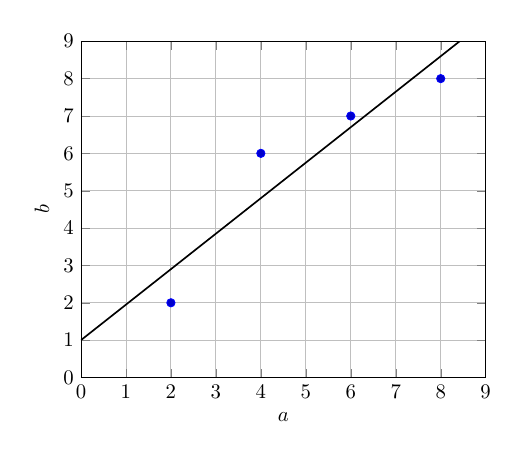
\begin{tikzpicture}[scale=0.75]
\begin{axis}[xlabel=$a$, ylabel=$b$, xmin=0, xmax=9, ymin=0, ymax=9,
             xtick={0,1,...,9}, ytick={0,1,...,9}, grid=major]
  \addplot+[only marks, mark=*] coordinates {(2,2) (4,6) (6,7) (8,8)};
  \addplot[thick, domain=0:9]{0.95 * x + 1};
\end{axis}
\end{tikzpicture}
\end{center}
\end{FigureBlock}
\FigureDescription{Horizontal axis $a$ runs from 0 to 9 with integer ticks;
vertical axis $b$ runs from 0 to 9 with integer ticks. The fitted line is
$b = 0.95a + 1$, passing through 1 at $a=0$ and 9.55 at $a=9$. It lies above
the first measured point and below the third.}

\begin{DataTable}[table/header-rows={1}]
\begin{center}
\begin{tabular}{|c|c|}
\hline
$a$ & $b$ \\
\hline
2 & 2 \\
4 & 6 \\
6 & 7 \\
8 & 8 \\
\hline
\end{tabular}
\end{center}
\end{DataTable}

\questionpart[10]
Set up the normal equations for the least-squares fit and solve for the slope
and intercept.

\begin{solution}
With $\mathbf{A}$ the matrix whose rows are $[a_i \;\; 1]$ and $\vec{b}$ the
vector of measurements, the normal equations are
$\mathbf{A}^{\!\top}\mathbf{A}\,\vec{x} = \mathbf{A}^{\!\top}\vec{b}$, giving a
slope of $0.95$ and an intercept of $1$.
\end{solution}

% ----------------------------------------------------------------------------
\question{Written Response}

\questionpart
State, in one sentence, why the residuals of a least-squares fit must be
orthogonal to the column space of $\mathbf{A}$.

% A tagged answer region, announced as such. The corpus used
% \framebox(470,42){} here, which is picture-mode and carries no semantics.
\answerbox[4\baselineskip]

\end{document}
"
% Hard-coding [sol] below would make `prob` a no-op, because both options would
% be processed and whichever \DeclareOption runs last wins.
%
% Open the result in a PDF reader and look at the bookmark/navigation pane:
% Homework 9 > Question 1 > Part (a) > Solution. Then run a screen reader over
% the figures: each is announced by its description, never by its contents.

\DocumentMetadata{
  lang       = en-US,
  pdfversion = 2.0,
  testphase  = {phase-III,math,table,graphic,firstaid},
}
\documentclass{latexa11y-assignment}

\usepackage{tikz}
\usepackage{pgfplots}
\pgfplotsset{compat=1.16}
\usepackage[american]{circuitikz}

\coursenumber{EECS 16A}
\coursename{Designing Information Devices and Systems I}
\semester{Spring 2026}
\university{UC Berkeley}

\begin{document}

\title{Homework 9}
\maketitle

\noindent
This homework is due Friday, April 3, 2026, at 23:59. Self-grades are due
Monday, April 6, 2026, at 23:59.

% ----------------------------------------------------------------------------
\question{Capacitor Charge Sharing}

Two capacitors are connected through a switch. Before $t=0$ the switch $S_1$ is
open, capacitor $C_1$ is charged to $V_1(0) = 5$\,V, and $C_2$ is uncharged.

% The figure speaks ONLY the description below. The labels drawn inside the
% schematic are never announced.
\begin{AltOnly}{Two capacitors, C1 and C2, each connected from its own top node
to ground, with switch S1 joining the two top nodes. C1 carries voltage V1 and
C2 carries voltage V2, both positive at the top.}
\begin{center}
\begin{circuitikz}[scale=0.9]
  \draw (0, 0) node[ground]{}
    (0, 3) to [C=$C_1$, v=$V_1$] ++ (0, -3)
    (0, 3) to [switch, l=$S_1$] ++ (6, 0)
          to [C=$C_2$, v=$V_2$] ++ (0, -3)
    node[ground]{};
\end{circuitikz}
\end{center}
\end{AltOnly}

\questionpart[5]
Express the total charge stored on both capacitors immediately before the
switch closes.

\begin{solution}
Only $C_1$ is charged, so $Q_{\text{total}} = C_1 V_1(0)$.
\end{solution}

\questionpart[5]
Find the steady-state voltage across both capacitors after the switch closes.

\begin{solution}
Charge is conserved and the two capacitors share a node, so they settle to a
common voltage
\[
  V_\infty = \frac{C_1 V_1(0)}{C_1 + C_2}.
\]
\end{solution}

% ----------------------------------------------------------------------------
\question{Least Squares Fit}

The table below records four measurements. A best-fit line has already been
drawn through them.

% Short /Alt plus a visible long description and a real data table: the tier
% for a figure whose data cannot fit in one spoken sentence.
\begin{FigureBlock}[alt={Scatter plot of b against a on axes running 0 to 9,
with four measured points and a straight best-fit line.}]
\begin{center}
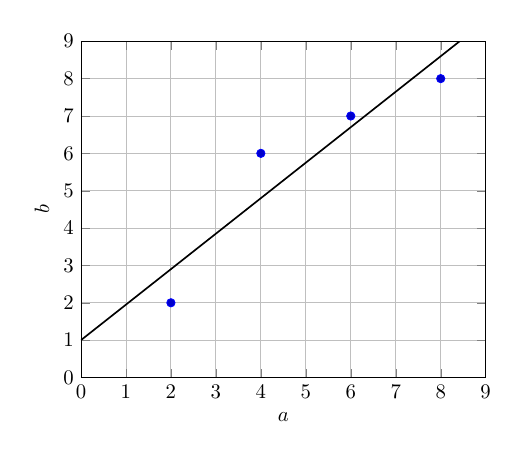
\begin{tikzpicture}[scale=0.75]
\begin{axis}[xlabel=$a$, ylabel=$b$, xmin=0, xmax=9, ymin=0, ymax=9,
             xtick={0,1,...,9}, ytick={0,1,...,9}, grid=major]
  \addplot+[only marks, mark=*] coordinates {(2,2) (4,6) (6,7) (8,8)};
  \addplot[thick, domain=0:9]{0.95 * x + 1};
\end{axis}
\end{tikzpicture}
\end{center}
\end{FigureBlock}
\FigureDescription{Horizontal axis $a$ runs from 0 to 9 with integer ticks;
vertical axis $b$ runs from 0 to 9 with integer ticks. The fitted line is
$b = 0.95a + 1$, passing through 1 at $a=0$ and 9.55 at $a=9$. It lies above
the first measured point and below the third.}

\begin{DataTable}[table/header-rows={1}]
\begin{center}
\begin{tabular}{|c|c|}
\hline
$a$ & $b$ \\
\hline
2 & 2 \\
4 & 6 \\
6 & 7 \\
8 & 8 \\
\hline
\end{tabular}
\end{center}
\end{DataTable}

\questionpart[10]
Set up the normal equations for the least-squares fit and solve for the slope
and intercept.

\begin{solution}
With $\mathbf{A}$ the matrix whose rows are $[a_i \;\; 1]$ and $\vec{b}$ the
vector of measurements, the normal equations are
$\mathbf{A}^{\!\top}\mathbf{A}\,\vec{x} = \mathbf{A}^{\!\top}\vec{b}$, giving a
slope of $0.95$ and an intercept of $1$.
\end{solution}

% ----------------------------------------------------------------------------
\question{Written Response}

\questionpart
State, in one sentence, why the residuals of a least-squares fit must be
orthogonal to the column space of $\mathbf{A}$.

% A tagged answer region, announced as such. The corpus used
% \framebox(470,42){} here, which is picture-mode and carries no semantics.
\answerbox[4\baselineskip]

\end{document}
"
% Hard-coding [sol] below would make `prob` a no-op, because both options would
% be processed and whichever \DeclareOption runs last wins.
%
% Open the result in a PDF reader and look at the bookmark/navigation pane:
% Homework 9 > Question 1 > Part (a) > Solution. Then run a screen reader over
% the figures: each is announced by its description, never by its contents.

\DocumentMetadata{
  lang       = en-US,
  pdfversion = 2.0,
  testphase  = {phase-III,math,table,graphic,firstaid},
}
\documentclass{latexa11y-assignment}

\usepackage{tikz}
\usepackage{pgfplots}
\pgfplotsset{compat=1.16}
\usepackage[american]{circuitikz}

\coursenumber{EECS 16A}
\coursename{Designing Information Devices and Systems I}
\semester{Spring 2026}
\university{UC Berkeley}

\begin{document}

\title{Homework 9}
\maketitle

\noindent
This homework is due Friday, April 3, 2026, at 23:59. Self-grades are due
Monday, April 6, 2026, at 23:59.

% ----------------------------------------------------------------------------
\question{Capacitor Charge Sharing}

Two capacitors are connected through a switch. Before $t=0$ the switch $S_1$ is
open, capacitor $C_1$ is charged to $V_1(0) = 5$\,V, and $C_2$ is uncharged.

% The figure speaks ONLY the description below. The labels drawn inside the
% schematic are never announced.
\begin{AltOnly}{Two capacitors, C1 and C2, each connected from its own top node
to ground, with switch S1 joining the two top nodes. C1 carries voltage V1 and
C2 carries voltage V2, both positive at the top.}
\begin{center}
\begin{circuitikz}[scale=0.9]
  \draw (0, 0) node[ground]{}
    (0, 3) to [C=$C_1$, v=$V_1$] ++ (0, -3)
    (0, 3) to [switch, l=$S_1$] ++ (6, 0)
          to [C=$C_2$, v=$V_2$] ++ (0, -3)
    node[ground]{};
\end{circuitikz}
\end{center}
\end{AltOnly}

\questionpart[5]
Express the total charge stored on both capacitors immediately before the
switch closes.

\begin{solution}
Only $C_1$ is charged, so $Q_{\text{total}} = C_1 V_1(0)$.
\end{solution}

\questionpart[5]
Find the steady-state voltage across both capacitors after the switch closes.

\begin{solution}
Charge is conserved and the two capacitors share a node, so they settle to a
common voltage
\[
  V_\infty = \frac{C_1 V_1(0)}{C_1 + C_2}.
\]
\end{solution}

% ----------------------------------------------------------------------------
\question{Least Squares Fit}

The table below records four measurements. A best-fit line has already been
drawn through them.

% Short /Alt plus a visible long description and a real data table: the tier
% for a figure whose data cannot fit in one spoken sentence.
\begin{FigureBlock}[alt={Scatter plot of b against a on axes running 0 to 9,
with four measured points and a straight best-fit line.}]
\begin{center}
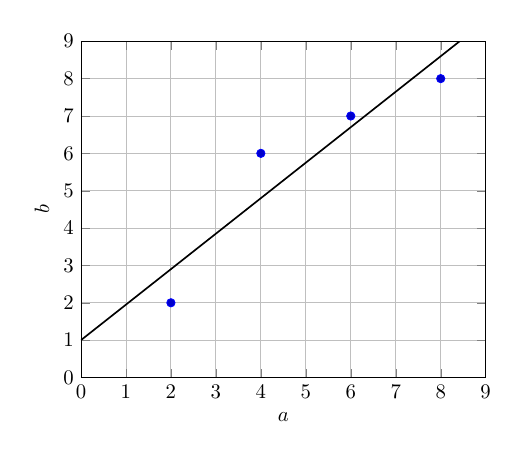
\begin{tikzpicture}[scale=0.75]
\begin{axis}[xlabel=$a$, ylabel=$b$, xmin=0, xmax=9, ymin=0, ymax=9,
             xtick={0,1,...,9}, ytick={0,1,...,9}, grid=major]
  \addplot+[only marks, mark=*] coordinates {(2,2) (4,6) (6,7) (8,8)};
  \addplot[thick, domain=0:9]{0.95 * x + 1};
\end{axis}
\end{tikzpicture}
\end{center}
\end{FigureBlock}
\FigureDescription{Horizontal axis $a$ runs from 0 to 9 with integer ticks;
vertical axis $b$ runs from 0 to 9 with integer ticks. The fitted line is
$b = 0.95a + 1$, passing through 1 at $a=0$ and 9.55 at $a=9$. It lies above
the first measured point and below the third.}

\begin{DataTable}[table/header-rows={1}]
\begin{center}
\begin{tabular}{|c|c|}
\hline
$a$ & $b$ \\
\hline
2 & 2 \\
4 & 6 \\
6 & 7 \\
8 & 8 \\
\hline
\end{tabular}
\end{center}
\end{DataTable}

\questionpart[10]
Set up the normal equations for the least-squares fit and solve for the slope
and intercept.

\begin{solution}
With $\mathbf{A}$ the matrix whose rows are $[a_i \;\; 1]$ and $\vec{b}$ the
vector of measurements, the normal equations are
$\mathbf{A}^{\!\top}\mathbf{A}\,\vec{x} = \mathbf{A}^{\!\top}\vec{b}$, giving a
slope of $0.95$ and an intercept of $1$.
\end{solution}

% ----------------------------------------------------------------------------
\question{Written Response}

\questionpart
State, in one sentence, why the residuals of a least-squares fit must be
orthogonal to the column space of $\mathbf{A}$.

% A tagged answer region, announced as such. The corpus used
% \framebox(470,42){} here, which is picture-mode and carries no semantics.
\answerbox[4\baselineskip]

\end{document}
